\section{Experiments}
\label{sec:experiments}

We evaluate on ten configurations spanning six families: Pythia-1.4B/6.9B, OLMo-1B, Qwen2.5-1.5B-Instruct (rewrite/continuation), Qwen2.5-1.5B (base), Qwen2.5-7B, LLaMA-3.1-8B, Mistral-7B, and Gemma-2-2B.
Unless noted, all experiments use the OBD-LightGBM classifier with 15 features (Section~\ref{sec:method}), 5{,}000 C4 texts per depth level (depths 0--5).

%% ====================================================================
\subsection{The Discrimination Boundary}
\label{sec:kstar_boundary}

\begin{figure}[t]
\centering
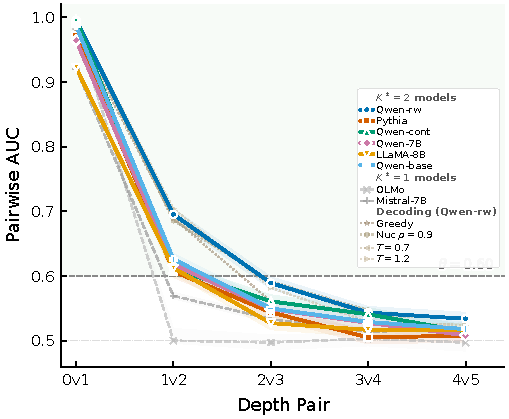
\includegraphics[width=\columnwidth]{figures/fig2_auc_decay.pdf}
\caption{Pairwise $\auc$ decay across adjacent depth pairs (0v1, 1v2, \ldots, 4v5) for model-mode configurations (solid) and decoding strategies (dashed); shaded bands show bootstrap 95\% CIs. Horizontal dashed line: $\theta = 0.60$.}
\label{fig:auc_decay}
\end{figure}

\begin{table*}[t]
\centering
\small
\caption{Pairwise $\auc$ for adjacent depth pairs with bootstrap 95\% CIs and permutation $p$-values for boundary rows.
$\Kempirical = 2$ requires 1v2 $\auc > \theta{=}0.60$ and 2v3 $\auc < \theta$; CIs quantify boundary uncertainty.
Extended results (all models) in Table~\ref{tab:kstar_ci_extended}.}
\label{tab:kstar_ci}
\resizebox{\textwidth}{!}{%
\begin{tabular}{lcccccccccc}
\toprule
 & \multicolumn{2}{c}{Qwen-rw} & \multicolumn{2}{c}{Pythia} & \multicolumn{2}{c}{OLMo} & \multicolumn{2}{c}{Qwen-cont} & \multicolumn{2}{c}{Qwen-7B\rlap{$^\ddagger$}} \\
\cmidrule(lr){2-3}\cmidrule(lr){4-5}\cmidrule(lr){6-7}\cmidrule(lr){8-9}\cmidrule(lr){10-11}
 & $\auc$ & 95\% CI & $\auc$ & 95\% CI & $\auc$ & 95\% CI & $\auc$ & 95\% CI & $\auc$ & 95\% CI \\
\midrule
0v1 & .9956 & & .9722 & & .9861 & & .9971 & & .9644 & [.961,\,.967] \\
1v2 & .6955 & [.686,\,.704]\rlap{$^*$} & .6074 & [.598,\,.617]\rlap{$^*$} & .5001 & [.496,\,.519] & .6112 & [.602,\,.621]\rlap{$^*$} & .6178 & [.608,\,.626]\rlap{$^*$} \\
2v3 & .5893 & [.580,\,.599] & .5440 & [.534,\,.554] & .4973 & [.486,\,.509] & .5609 & [.551,\,.571] & .5492 & [.539,\,.559] \\
3v4 & .5435 & & .5051 & & .5034\rlap{$^\S$} & & .5409 & & .5276 & \\
4v5 & .5340 & & .5079 & & .4971 & & .5141 & & .5085 & \\
\bottomrule
\multicolumn{11}{l}{\footnotesize $^*$Permutation $p < 0.001$ for all starred boundary comparisons ($\auc > \theta$).} \\
\multicolumn{11}{l}{\footnotesize $^\ddagger$Generator: Qwen2.5-7B (fp16); scorer: Qwen2.5-1.5B.} \\
\multicolumn{11}{l}{\footnotesize $^\S$OLMo 2v3 (0.497) $<$ 3v4 (0.503): non-monotonic reversal within noise ($\Delta = 0.006$).} \\
\multicolumn{11}{l}{\footnotesize Full results for all 10 configurations (including LLaMA-8B, Mistral-7B, Qwen-base, Gemma-2-2B, and Pythia-6.9B) in Table~\ref{tab:kstar_ci_extended}.}
\end{tabular}}
\end{table*}

Table~\ref{tab:kstar_ci} and Figure~\ref{fig:auc_decay} show $\Kempirical \leq 2$ across all 10 configurations: 6/10 yield $\Kempirical{=}2$ (1v2 $\auc$: 0.607--0.696; $p < 0.001$), while 4/10 yield $\Kempirical{=}1$ (1v2 $\auc$: 0.500--0.598; Section~\ref{sec:boundary_cases}).
Across six architecture families, three (Qwen, Pythia, LLaMA) yield $\Kempirical{\geq}2$ in at least one configuration; the remaining three (OLMo, Gemma-2, Mistral) yield $\Kempirical{=}1$.
Pythia exhibits a scale-dependent split (1.4B: $\Kempirical{=}2$, 6.9B: $\Kempirical{=}1$); Qwen dominates the $\Kempirical{=}2$ count (4 of 6 configurations).
Under Bonferroni correction (99.5\% CIs; Table~\ref{tab:bonferroni_ci}), three of six $\Kempirical{=}2$ configurations retain significance; the three marginal cases (Pythia-1.4B, Qwen-cont, LLaMA-8B; CI lower bounds 0.593--0.599) reflect narrow effect sizes rather than classification failure ($\Kempirical$ is robust to $\theta$ within $[0.59, 0.60]$; Figure~\ref{fig:kstar_theta}).
LLaMA-3.1-8B confirms $\Kempirical{=}2$ (0v1 $\auc = 0.9225$, 1v2 $\auc = 0.6123\;[0.603,\,0.622]$; CI lower bound above $\theta$; Table~\ref{tab:kstar_ci_extended}).
All four decoding strategies likewise yield $\Kempirical{=}2$ (Table~\ref{tab:s2_decoding}; Pythia-1.4B replication in Table~\ref{tab:s10_pythia_decoding}).
The 1v2 spread due to generation mode ($\Delta = 8.4$\,pp within Qwen) exceeds the spread across $\Kempirical{=}2$ continuation models ($\Delta = 1.9$\,pp).
Bootstrap resampling (1{,}000 iterations) confirms stability: 8/10 configurations yield identical $\Kempirical$ across all resamples (two boundary cases have CIs of width~1; the $\Kempirical \leq 2$ bound holds universally); together with the between-sample 5K-vs.-10K comparison (Table~\ref{tab:robustness_10k}), this bounds $\Kempirical$ uncertainty from complementary angles (Table~\ref{tab:bootstrap_kstar}; per-fold AUCs in Table~\ref{tab:s8_cv_folds}).
The two exceptions, Gemma-2B C4 and LLaMA-8B Wikipedia (92.7\% and 94.3\% modal-$\Kempirical$ consistency), have 1v2 AUC within 1\,pp of $\theta$; their bootstrap instability predicts the between-sample drift in Table~\ref{tab:robustness_10k}; boundary proximity rather than sample size drives the observed variability.

\paragraph{Scale and instruction-tuning invariance.}
$\Kempirical{=}2$ persists from 1.5B through 8B: Qwen-7B (1v2 $\auc = 0.6178$ $[0.608, 0.626]$) and LLaMA-3.1-8B (1v2 $\auc = 0.6123$) both exceed $\theta$, despite progressively reduced 0v1 signal (0.9644 and 0.9225 vs.\ $> 0.97$ at $\leq$1.5B).
A base-vs.-instruct ablation at 1.5B likewise yields $\Kempirical = 2$ (1v2 $\auc = 0.626$); the boundary is not an instruction-tuning artifact.

\begin{figure*}[t]
\centering
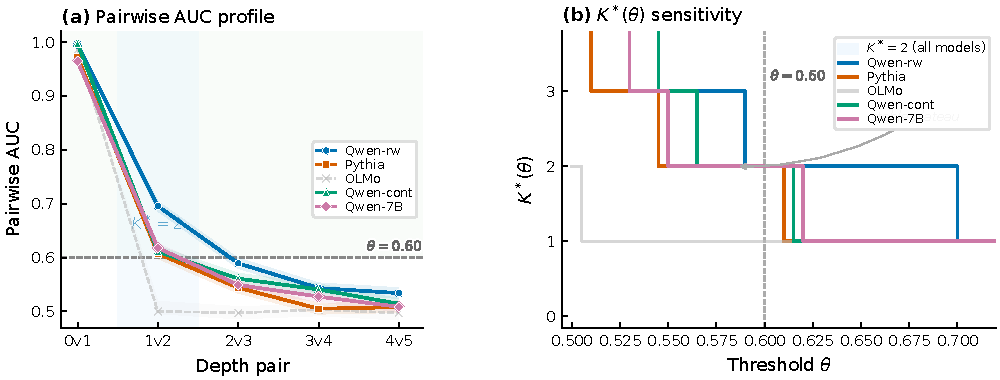
\includegraphics[width=0.75\textwidth]{figures/fig_kstar_theta.pdf}
\caption{$\Kempirical(\theta)$ sensitivity curve for five configurations. $\Kempirical$: maximum discriminable depth; $\theta$: AUC decision threshold. Four of five configurations yield $\Kempirical{=}2$ at $\theta{=}0.60$ (dashed line); OLMo yields $\Kempirical{=}1$. At $\theta{=}0.70$, all drop to $\Kempirical{=}1$.}
\label{fig:kstar_theta}
\end{figure*}

Figure~\ref{fig:kstar_theta} displays the sensitivity surface across $\theta \in [0.50, 0.70]$: four of five configurations shown yield $\Kempirical \geq 2$ for $\theta \leq 0.60$ (OLMo: $\Kempirical = 1$ throughout); at $\theta{=}0.55$, two Qwen configurations reach $\Kempirical = 3$; at $\theta{=}0.70$, all drop to $\Kempirical = 1$.
$\Kempirical{=}2$ is stable across $\theta \in [0.59, 0.60]$; at $\theta{=}0.61$, one borderline case (Pythia-1.4B) drops to $\Kempirical{=}1$.

%% ====================================================================
\subsection{Cross-Model Transfer}
\label{sec:transfer}

\begin{figure}[!t]
\centering
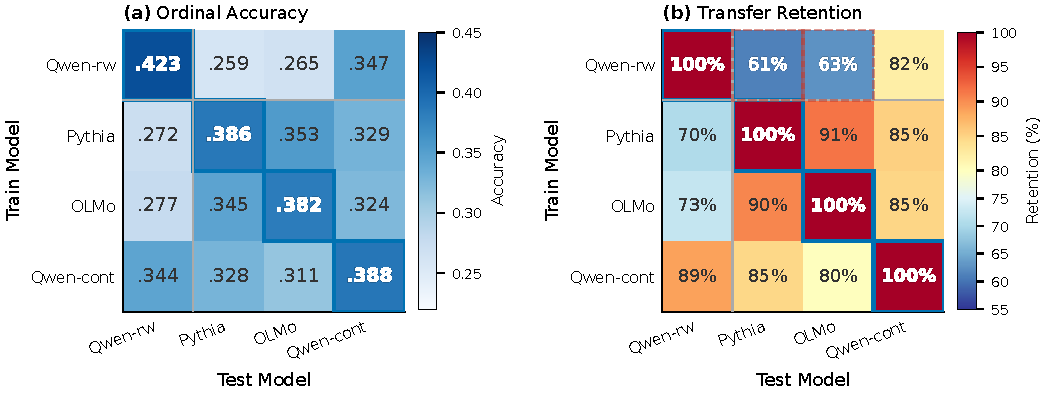
\includegraphics[width=\columnwidth]{figures/fig3_transfer_heatmap.pdf}
\vspace{-6pt}
\caption{Cross-model transfer heatmap (three continuation-mode models plus Qwen-rewrite). \textbf{(a)} 6-class ordinal accuracy when trained on the row model and evaluated on the column model; diagonal entries (highlighted) are in-domain baselines. \textbf{(b)} Retention rate (off-diagonal accuracy divided by in-domain accuracy). Continuation-mode pairs retain 80--92\%; Qwen-rw transfers at 61--63\% to other architectures but 82\% to Qwen-cont, consistent with a mode-specific artifact.}
\label{fig:transfer_heatmap}
\end{figure}

Continuation-mode classifiers transfer well across generators (Figure~\ref{fig:transfer_heatmap}; full matrix in Table~\ref{tab:s1_transfer}): Pythia$\leftrightarrow$OLMo retains 90--92\%, Qwen-cont$\leftrightarrow$Pythia 84--85\%, Qwen-cont$\leftrightarrow$OLMo 80--85\%.
Cross-scale transfer from Gemma-2-27B retains $>$100\% accuracy on 1B--8B models (101.3\% avg; ${\leq}$1.5B$\to$27B: 76.5\%); larger models may learn a universal depth-feature superset (Table~\ref{tab:gemma27b_transfer}; filtering validation in Table~\ref{tab:gemma27b_filtering}).
Qwen-rewrite classifiers transfer at 61--63\% to Pythia and OLMo but retain 82\% to Qwen-cont; cross-architecture degradation reflects a mode-specific artifact, while the within-family retention points to a Qwen-specific component layered on top.

\paragraph{Cross-scorer validation.}
Replacing the self-scorer with Pythia-1.4B or OLMo-1B preserves feature rankings ($\rho > 0.90$) but attenuates absolute discriminability at the boundary (Table~\ref{tab:crossscorer}; $\Kempirical$ comparison in Table~\ref{tab:s13_scorer_sensitivity}).
Feature ranking independence is a strong result: the same features dominate under all scorers (Table~\ref{tab:crossscorer}).
$\Kempirical$ agreement, however, is signal-strength dependent: Qwen-rewrite (strong signal, 1v2 $\auc = 0.696$) retains $\Kempirical{=}2$ under all scorers, but Qwen-continuation (marginal, 1v2 $\auc = 0.611$, only 0.011 above $\theta$) drops to $\Kempirical{=}1$ (Pythia: $0.5923$; OLMo: $0.5858$).
A three-way analysis of variance (ANOVA) (Generator $\times$ Scorer $\times$ Depth-Pair; Table~\ref{tab:anova_crossscorer}) confirms a statistically significant but modest Scorer main effect ($\eta^2_p{=}.192$, $p < .001$) and a significant Generator$\times$Scorer interaction ($\eta^2_p{=}.170$); absolute AUC values are thus scorer-dependent even when $\Kempirical$ classifications largely agree.

%% ====================================================================
\subsection{Feature Ordering and Generation Mode}
\label{sec:feature_degradation}
\label{sec:generation_mode}

Among continuation-mode models, single-feature $\auc$ rankings are highly correlated ($\rho \geq 0.85$; Table~\ref{tab:top_features}).
The top-3 features (\texttt{surp\_d1\_std}, \texttt{surp\_std}, \texttt{surp\_d2\_std}) are shared across all three families: autoregressive generation progressively damps surprisal variability.
Qwen-rewrite diverges (\texttt{freq\_entropy} dominates), consistent with its low cross-architecture transfer (61--63\% to Pythia/OLMo; 82\% within Qwen).
Within Qwen, rewrite yields 1v2 $\auc = 0.6955$ vs.\ continuation's $0.6112$ ($\Delta = +8.4$\,pp); continuation mode is therefore recommended as the canonical condition.

%% ====================================================================
\subsection{Neural Probe}
\label{sec:neural_probe}

Replacing the 15D features with frozen encoder hidden states (multilayer perceptron (MLP) probe; Table~\ref{tab:neural_probe_crossmodel}; architecture in Table~\ref{tab:s7_neural_probe}), Qwen achieves $\Kempirical^{\text{neural}} = 3$ (2v3 $\auc = 0.6159$), while Pythia remains at $\Kempirical^{\text{neural}} = 2$ ($\auc_{2v3} = 0.5963$); OLMo yields $\Kempirical^{\text{neural}} = 1$ (1v2 $\auc = 0.5054$, consistent with its 15D boundary).
We hypothesize that the Qwen-only elevation reflects self-familiarity artifacts, consistent with the poor transfer observed in Section~\ref{sec:transfer}; the 15D features yield $\Kempirical = 2$ for most families (OLMo: $\Kempirical = 1$).

\begin{table}[t]
\centering
\footnotesize
\caption{Neural probe pairwise AUC using frozen-encoder MLP. Each cell reports AUC for classifying depth $d$ vs.\ $d{+}1$ text. $\Kempirical^{\text{neural}}$: maximum depth where AUC exceeds $\theta = 0.60$.}
\label{tab:neural_probe_crossmodel}
\resizebox{\columnwidth}{!}{%
\begin{tabular}{lccc}
\toprule
\textbf{Model} & \textbf{2v3 $\auc$} & \textbf{95\% CI} & $\Kempirical^{\text{neural}}$ \\
\midrule
Qwen-1.5B  & 0.6159 & $[0.610,\,0.622]$ & 3 \\
Pythia-1.4B & 0.5963 & $[0.589,\,0.603]$ & 2 \\
OLMo-1B    & 0.5056 & $[0.497,\,0.516]$ & 1\rlap{$^\dagger$} \\
\bottomrule
\multicolumn{4}{l}{\footnotesize $^\dagger$OLMo 1v2 $\auc = 0.5054$ (below $\theta$); $\Kempirical^{\text{neural}} = 1$.}
\end{tabular}}
\end{table}

%% ====================================================================
\subsection{Cross-Domain Variation}
\label{sec:cross_domain}

The preceding experiments use C4 (general web text).
To test domain dependence, we evaluate on Wikipedia ($n{=}5{,}000$) and arXiv abstracts ($n{=}2{,}200$) across five architecture families (Table~\ref{tab:s12_domain_ablation}).
Wikipedia yields $\Kempirical{=}2$ for Qwen-1.5B (1v2 $\auc = 0.619$; Table~\ref{tab:domain_kstar}), but $\Kempirical{=}1$ for LLaMA-8B and Mistral-7B (1v2 $\auc = 0.592,\,0.558$; both below $\theta$).
Qwen-1.5B, Pythia-1.4B, LLaMA-3.1-8B, and Mistral-7B yield $\Kempirical{=}3$ for arXiv (Table~\ref{tab:domain_kstar}): 2v3 $\auc = 0.643\;[0.628,\,0.658]$, $0.655\;[0.634,\,0.662]$, $0.622\;[0.605,\,0.635]$, and $0.628$ respectively (permutation $p < 0.001$); structured academic text thus permits discrimination to greater depth independently of architecture.
OLMo-1B is the sole exception ($\Kempirical{=}1$ across all domains; cross-scorer validated, $p{=}0.510$); Mistral-7B exhibits a monotonic staircase (Wiki${=}$1, C4${=}$1, Code${=}$2, arXiv${=}$3); $\Kempirical$ is domain-determined.
The elevated signal reflects higher per-generation distributional shift (1v2 Jensen--Shannon divergence (JSD) $= 0.077$ vs.\ ${\sim}0.01$ for C4; Figure~\ref{fig:jsd_decay}), as formulaic structure amplifies deviation from domain norms; a multi-source pooled classifier confirms that the arXiv ceiling is text-intrinsic (Appendix~\ref{sec:arxiv_multi_source}).

\begin{figure}[t]
\centering
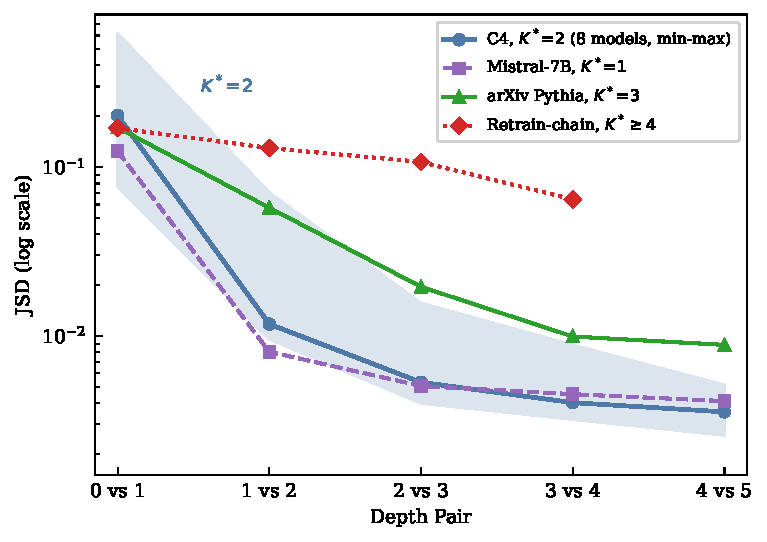
\includegraphics[width=\columnwidth]{figures/fig_jsd_decay.pdf}
\caption{JSD between adjacent depth pairs (log scale). C4 band (blue): min-max over 8 $\Kempirical{=}2$ configurations (4~model-mode pairs $+$ 4~Pythia decoding variants; $\Kempirical{=}1$ models excluded). arXiv (green) sustains signal to depth~3; retrain-chain (red) remains elevated.}
\label{fig:jsd_decay}
\end{figure}
We additionally evaluate on CodeSearchNet Python ($n{=}5{,}000$, continuation mode); all five tested models (Qwen-1.5B, Qwen-7B, LLaMA-8B, Mistral-7B, OLMo-1B) yield $\Kempirical \leq 2$ (Table~\ref{tab:domain_kstar}), matching the C4 baseline.

\begin{table}[t]
\centering
\footnotesize
\caption{Cross-domain $\Kempirical$ comparison. $\Kempirical{\leq}2$ for C4 and Code (most families $\Kempirical{=}2$; OLMo-1B: 1); $\Kempirical{=}3$ for arXiv (four families); Wikipedia varies (1--2). Mistral-7B spans all four domains, exhibiting a monotonic staircase. Bonferroni-corrected 99.5\% CI reported for the boundary pair where available (2v3 for $\Kempirical{=}3$; 1v2 otherwise).}
\label{tab:domain_kstar}
\resizebox{\columnwidth}{!}{%
\begin{tabular}{llcccc}
\toprule
\textbf{Domain} & \textbf{Model} & \textbf{1v2 $\auc$} & \textbf{2v3 $\auc$} & \textbf{Bonf CI} & $\Kempirical$ \\
\midrule
arXiv & Qwen-1.5B\rlap{$^\dagger$}  & .858 & .643 & [.628,\,.658] & 3 \\
arXiv & Pythia-1.4B & .805 & .655 & [.634,\,.662] & 3 \\
arXiv & LLaMA-8B    & .845 & .622 & [.605,\,.635] & 3 \\
arXiv & Mistral-7B  & .820 & .628 & --- & 3 \\
arXiv & OLMo-1B\rlap{$^\S$}    & .500 & .497 & [.483,\,.517] & 1 \\
C4    & Qwen-1.5B\rlap{$^\dagger$}  & .626 & .550 & --- & 2 \\
C4    & Mistral-7B  & .570 & .534 & --- & 1 \\
Code  & Qwen-1.5B\rlap{$^\dagger$}  & .738 & .530 & --- & 2 \\
Code  & Qwen-7B    & .727 & .537 & [.715,\,.739] & 2 \\
Code  & LLaMA-8B   & .739 & .511 & --- & 2 \\
Code  & Mistral-7B  & .615 & .529 & [.602,\,.628] & 2 \\
Code  & OLMo-1B\rlap{$^\S$}    & .557 & .500 & --- & 1 \\
Wiki  & Qwen-1.5B\rlap{$^\dagger$}  & .619 & .550 & --- & 2 \\
Wiki  & LLaMA-8B\rlap{$^\ddagger$}  & .592 & .538 & [.579,\,.605] & 1 \\
Wiki  & Mistral-7B  & .558 & .519 & [.543,\,.572] & 1 \\
\bottomrule
\multicolumn{6}{l}{\footnotesize $^\dagger$Qwen2.5-1.5B (base, continuation mode).} \\
\multicolumn{6}{l}{\footnotesize $^\ddagger$Marginal: point estimate $< \theta$; CI upper bound crosses 0.60.} \\
\multicolumn{6}{l}{\footnotesize $^\S$Sole exception: $K^*{=}1$ across all domains; cross-scorer validated ($p{=}0.510$, n.s.).}
\end{tabular}}
\end{table}

\paragraph{Robustness.}
\label{sec:robustness}
$\Kempirical{=}2$ holds across segment lengths of 128, 256, and 512 tokens (Table~\ref{tab:s11_length_ablation}; token-level statistics in Table~\ref{tab:token_length}); at 512 tokens the 1v2 CI lower bound falls marginally below $\theta$ but 2v3 remains well below $\theta$ at all lengths ($\leq 0.572$).
Seed robustness testing (seed $= 123$ vs.\ primary $= 42$; Table~\ref{tab:seed_robustness}) confirms $\Kempirical$ stability in 2/3 configurations; the one marginal shift (Qwen-Wikipedia $\Kempirical{=}2 \to 3$, 2v3 $\auc = 0.607$) has one of five folds below $\theta$.
The ${\pm}9$\,pp absolute AUC variation across seeds strengthens the case for threshold-based $\Kempirical$ over raw AUC comparisons.

%% ====================================================================
\subsection{Binary Detector Confidence}
\label{sec:binary_confidence}

Binary detectors (DivEye~\cite{basani2026diveye}, Binoculars~\cite{hans2024binoculars}) provide no depth signal beyond the human-vs.-machine boundary: $\Kempirical^{\text{binary}} \leq 1$, with moderate rank correlations ($|\rho| = 0.06$--$0.46$) driven entirely by the 0v1 gap (Table~\ref{tab:s9_binary_spearman}).
